\subsection{Kraftfelder}
\label{mdforcefields}

Zentrales Element molekulardynamischer Methoden sind Kraftfelder~$\vec F(X)$, auch Potentiale~$V(X)$ genannt, welche die Interaktionen der simulierten Teilchen beschreiben.
Für verschiedene Materialien existieren spezielle Potentialformulierungen, die für unterschiedliche Elemente wiederum eigene Potentialparametrisierungen in Form von Potentialdateien zur Verfügung stellen.
Im Folgenden soll eine Auswahl dieser Potentialformulierungen kurz in ihrer Funktionsweise vorgestellt werden.

\subsubsection{Paar-Potentiale}

Das einfachste MD-Potential ist das Paarpotential, welches Interaktionen zwischen jeweils zwei benachbarten Atomen modelliert.
Damit vereinfacht sich die Energie des Gesamtsystems auf Summen des Potentiales $V$ über alle Paare von Atomen in Abhängigkeit ihres Abstandes $r_ij$:
\begin{equation}
  \vec F_{ij}(r_{ij}) = \vec\nabla V(r_{ij})
\end{equation}
\begin{equation}
  E = \sum_i\sum_{j \neq i}{V(r_{ij})}
\end{equation}

Stellvertretend steht das Lennard-Jones-Potential zur Darstellung von allgemeinen Fluiden:
\begin{equation}
  V_\text{LJ}(r_{ij}) = 4 \epsilon \left[\left(\frac{\sigma}{r_{ij}}\right)^{12} - \left(\frac{\sigma}{r_{ij}}\right)^{6}\right]
\end{equation}
Weitere Paarpotentiale wie etwa das mit dem Lennard-Jones-Potential verwandte Bucking\-ham-Potential nehmen aufgrund unterschiedlicher Anwendungsgebiete andere Formen an (Abbildung~\ref{fig:mdpairpotentials}).
Allen Paar-Potentialen ist gemein, eine rein radiale Abhängigkeit $V(r_ij)$ zu besitzen, die oftmals einen charakteristischen Bindungsabstand in Abhängigkeit der Parameter bildet, welcher sich als Minimum in den Potentialen äußert.
Unterhalb dieses Radius' dominiert ein repulsiver Term, wo hingegen oberhalb davon ein leicht attraktiver Term vorherrscht, der sich für große Radien einem konstanten Wert annähert und deshalb mit einem Cutoff-Radius $r_\text{cut}$ versehen ist.

\begin{figure}
  \centering
  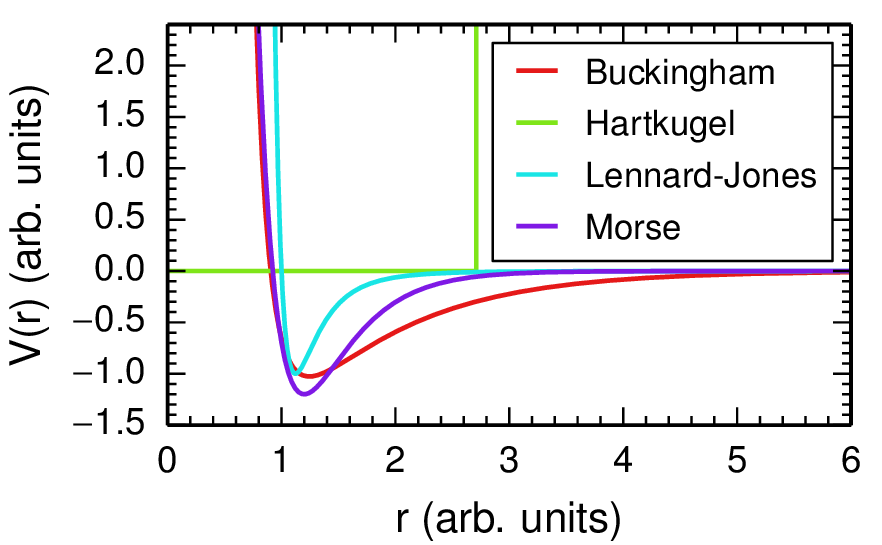
\includegraphics[width=0.5\textwidth]{mdpotplot}
  \caption{Auswahl einfacher molekulardynamischer Paarpotentiale}
  \label{fig:mdpairpotentials}
\end{figure}

\todo{Beleg, Zitat, Nachweis}Zwar zeigen Paarpotentiale gute thermodynamische Eigenschaften bei geringem Rechenaufwand, doch können sie aufgrund ihrer simplen Formulierung keine atomistischen Strukturen verlässlich vorhersagen.

\subsubsection{N-Teilchen-Potentiale}

N-Teilchen-Potentiale erweitern Paarpotentiale um weitere Terme, die von der Position einer festen Anzahl an Teilchen abhängen.
Damit können beispielsweise Winkel- und Torsionsabhängigkeiten wiedergegeben werden.

\begin{equation}
  E = \sum_i\sum_{j \neq i}{V_2\left(r_{ij}\right)} + \sum_i\sum_{j \neq i}\sum_{\substack{k \neq i \\ k \neq j}}{V_3\left(r_{ij}, r_{ik}, \theta_{ijk}\right)} + \dots
\end{equation}
Obwohl sich mit N-Teilchen-Potentialen komplexere Systeme betrachten lassen, zeigen sie die gleichen Schwachstellen wie Paarpotentiale, benötigen aber eine größere Anzahl an Parametern.
Zwar gibt es erfolgreiche Anwendungen für Biomoleküle\cite{case_amber_2005,brooks_charmm:_1983,brooks_charmm:_2009,berendsen_gromacs:_1995,hess_gromacs_2008}, die allerdings aufgrund ihrer \todo{Darstellung kovalenter und H-Bindungen, nicht anderer Beziehungen}Spezialisierung nicht auf andere Stoffsysteme wie Festkörper oder Oberflächen übertragbar sind.

\subsubsection{Embedded Atom Model}

Das Embedded Atom Model (EAM) besteht aus einem Paarpotential $V_{\alpha\beta}(r_{ij})$ für jedes Atom $i$ sowie einer Einbettungsfunktion $F_\alpha$, welche die Energie des Atomes in Abhängigkeit der angenäherten lokalen Elektronendichte $\rho_\beta(r_{ij})$ modelliert\cite{daw_embedded-atom_1984}.
\begin{equation}
  E = \sum_i\left[F_\alpha\left(\sum_{j\neq i}{\rho_\beta\left(r_{ij}\right)}\right) + \frac{1}{2}\sum_{j\neq i}{V_{\alpha\beta}\left(r_{ij}\right)}\right]
\end{equation}
So lassen sich metallische Bulksysteme und Oberflächen simulieren, für die $\alpha$ und $\beta$ verschiedene Spezies darstellen, doch führt die Formulierung für andere Systeme zwangsläufig zur Bildung von Clustern\todo{ggfs. erläutern oder durch Zitat belegen}.
Für eine Vielzahl an Metallen und Legierungen finden sich in Potentialdatenbanken fertige Parametrisierungen\cite{becker_interatomic_2014}, von denen viele zusätzlich zu den strukturellen auch thermodynamische Eigenschaften recht gut modellieren (Abschnitt~\ref{goldthermo}).

%% \subsubsection{Modified Embedded Atom Model}

Für Metalloxide und weitere Mischsysteme existiert eine Erweiterung in Form des Modified Embedded Atom Models\cite{baskes_modified_1992}, dem eine umfangreichere Formulierung der lokalen Elektronendichten zugrunde liegt.

%% Als Erweiterung des EAM-Potentials wurden MEAM-Potentiale entwickelt, die neben Metallen und Legierungen auch Metalloxide und andere Mischsysteme ermöglichen sollen\cite{baskes_modified_1992}.
%% Sie basieren auf der gleichen Funktionsweise, stellen die Einbettungsenergie aber in Abhängigkeit einer umfangreicheren Formulierung der lokalen Elektronendichte dar.
%% Aufgrund der umfangreichen Formulierung soll auf die ursprüngliche Publikation von Baskes\cite{baskes_modified_1992} verwiesen werden.

%% \begin{equation}
%%   E = \sum_i\left[F_\alpha\left(\bar{\rho_i}\right) + \frac{1}{2}\sum_{j\neq i}{V_{ij}\left(r_{ij}\right)}\right]
%% \end{equation}

\subsubsection{Reactive Force Fields}

Reaktive Kraftfelder (Reactive Force Fields, ReaxFF) wurden von \textsc{van Duin et al.}\cite{van_duin_reaxff:_2001} 2001 mit dem Ziel entwickelt, Reaktionen zwischen Molekülen mit molekulardynamischen Methoden beschreiben zu können.
Mangels expliziter Beschreibung der involvierten Elektronen war die Beschreibung von Bindungen zuvor nur mit Elektronenstrukturrechnungen möglich, denen aber eine obere Grenze von wenigen hundert Atomen gesetzt ist.
Durch Beschreibung der Über- und Unterkoordination der Atome innerhalb ihrer Nachbarschaft, zusätzlich zum Ladungsaustausch zwischen den Atomen, Van-der-Waals- und elektrostatischen Kräften, lassen sich mit der ReaxFF-Formulierung Bindungen während der Simulation dynamisch formen und lösen, wodurch die Simulation von Reaktionen ermöglicht wird.
Die Gesamtenergie $E_\text{system}$ des Systemes setzt sich aus den folgenden Summanden zusammen, über die Tabelle~\ref{tab:reaxenergies} einen kurzen Überblick gibt.
\begin{align}
  \label{reaxformulation}
  E_\text{system} =~& E_\text{bond} + E_\text{lp} + E_\text{over} + E_\text{under} + E_\text{val} + E_\text{pen} + E_\text{coa} + E_\text{C2} \\
  \nonumber  & + E_\text{tors} + E_\text{conj} + E_\text{H-bond} + E_\text{vdWaals} + E_\text{Coulomb}
\end{align}
Die meisten Terme werden über die Bindungsordnung berechnet, welche sich wiederum aus Beiträgen für $\sigma$-, $\pi$- und Doppel-$\pi$-Bindungen aus dem Bindungsabstand zusammen setzt.
Darüber hinaus werden einige Terme in der Nähe des Cutoff-Abstands sowie an Koordinations-Übergängen auf 0 gesenkt, um Diskontinuitäten zu vermeiden und einen fließenden Übergang zwischen Bindungszuständen zu ermöglichen.

\begin{table}
  \oddrowcolors
  \caption[Summanden der ReaxFF-Gesamtenergie]{
    Erläuterung der Summanden der ReaxFF-Gesamtenergie aus Gleichung~\ref{reaxformulation}\cite{van_duin_reaxff:_2001}
  }
  \label{tab:reaxenergies}
  \begin{tabularx}{\textwidth}{|llX|}
    \hline
    \textbf{Term}      & \textbf{Beitrag}            & \textbf{Kommentar}                            \\
    \hline
    $E_\text{bond}$    & Bindungsenergien            & Berechnung über Bindungsordnung               \\
    $E_\text{lp}$      & freie Elektronenpaare       & über Bindungsordnungssumme am Atomzentrum     \\
    $E_\text{over}$    & Überkoordinationen          & unter Ausschluss freier Elektronenpaare       \\
    $E_\text{under}$   & Unterkoordinationen         & nur bei unterkoordinierten $\pi$-Bindungen    \\
    $E_\text{val}$     & Bindungswinkel              & Optimum abhängig von Elektronenkonfiguration  \\
    $E_\text{pen}$     & Strafenergien               & Fehlerkorrektur bei Winkeln mit Doppelbindung \\
    $E_\text{coa}$     & Drei-Teilchen-Konjugationen & Stabilisierung von NO$_2$-Gruppen             \\
    $E_\text{C2}$      & Dreifachbindungskorrektur   & Stabilisierung der Dreifachbindung von C$_2$  \\
    $E_\text{tors}$    & Torsionsbarrieren           &                                               \\
    $E_\text{conj}$    & Vier-Teilchen-Konjugationen & Konjugation bei Kohlenwasserstoffen           \\
    $E_\text{H-bond}$  & Wasserstoffbrücken          &                                               \\
    $E_\text{vdWaals}$ & Van-der-Waals-Kräfte        &                                               \\
    $E_\text{Coulomb}$ & Coulomb-Kräfte              &                                               \\
    \hline
  \end{tabularx}
\end{table}

Aus den Termen des ReaxFF-Potentials geht hervor, dass es ursprünglich für Reaktionen von organischen Molekülen entwickelt wurde, doch hat es sich als vielseitig genug herausgestellt, auch eine Vielzahl anderer Materialien wie Kristalle und nichtorganische Verbindungen simulieren zu können.
Die einzige Abhängigkeit besteht zum Trainingssatz, also den Test-Strukturen, an deren Werte die Parametrisierung des Reax-Kraftfeldes angepasst wurde.
So kann die Parametrisierung in der Regel nur die Strukturen und Materialien zuverlässig wiedergeben, für die sie ursprünglich erstellt wurde.
Für darüber hinaus gehende Anwendungen ist \todo{in der Regel}eine aufwendige Anpassung der Parametersätze mittels geeigneter Trainingsstrukturen erforderlich.\todo{Zitat?}

In den letzten fünf Jahren haben Reactive Force Fields jedoch an Aufmerksamkeit gewonnen, so dass die Zahl verfügbarer spezialisierter Parametrisierungen stetig zunimmt.
Es gibt auch Bestrebungen, sich ergänzende ReaxFF-Parametrisierungen zu kombinieren und somit mit einer Parametrisierung eine große Zahl von Zielsystemen betrachten zu können.
Besonders in kommerzieller MD-Software\cite{biovia_materials_2014} wird so versucht, dem Nutzer ein umfassendes Paket für die Simulation beliebiger Strukturen zu präsentieren, ohne ihm aber die Grenzen der Vorhersagekraft des Parametersatzes erkenntlich zu machen.
